\section{Performance Evaluation \& Benchmarks}
\label{sec:benchmarks}

\subsection{Experimental Setup}
\label{subsec:exp_setup}
Performance benchmarks were conducted on a 64-bit multi-core platform running Python 3.13.5. The automated benchmarking pipeline is depicted in Fig. \ref{fig:bm_pipeline}. High-precision execution timings were collected using `time.perf_counter_ns()`, and peak memory allocation footprints were recorded via Python memory tracing APIs over 100 evaluation trials. Benchmark payload sizes ranged from 64 B to 1 MB.

\begin{figure}[htbp]
\centering
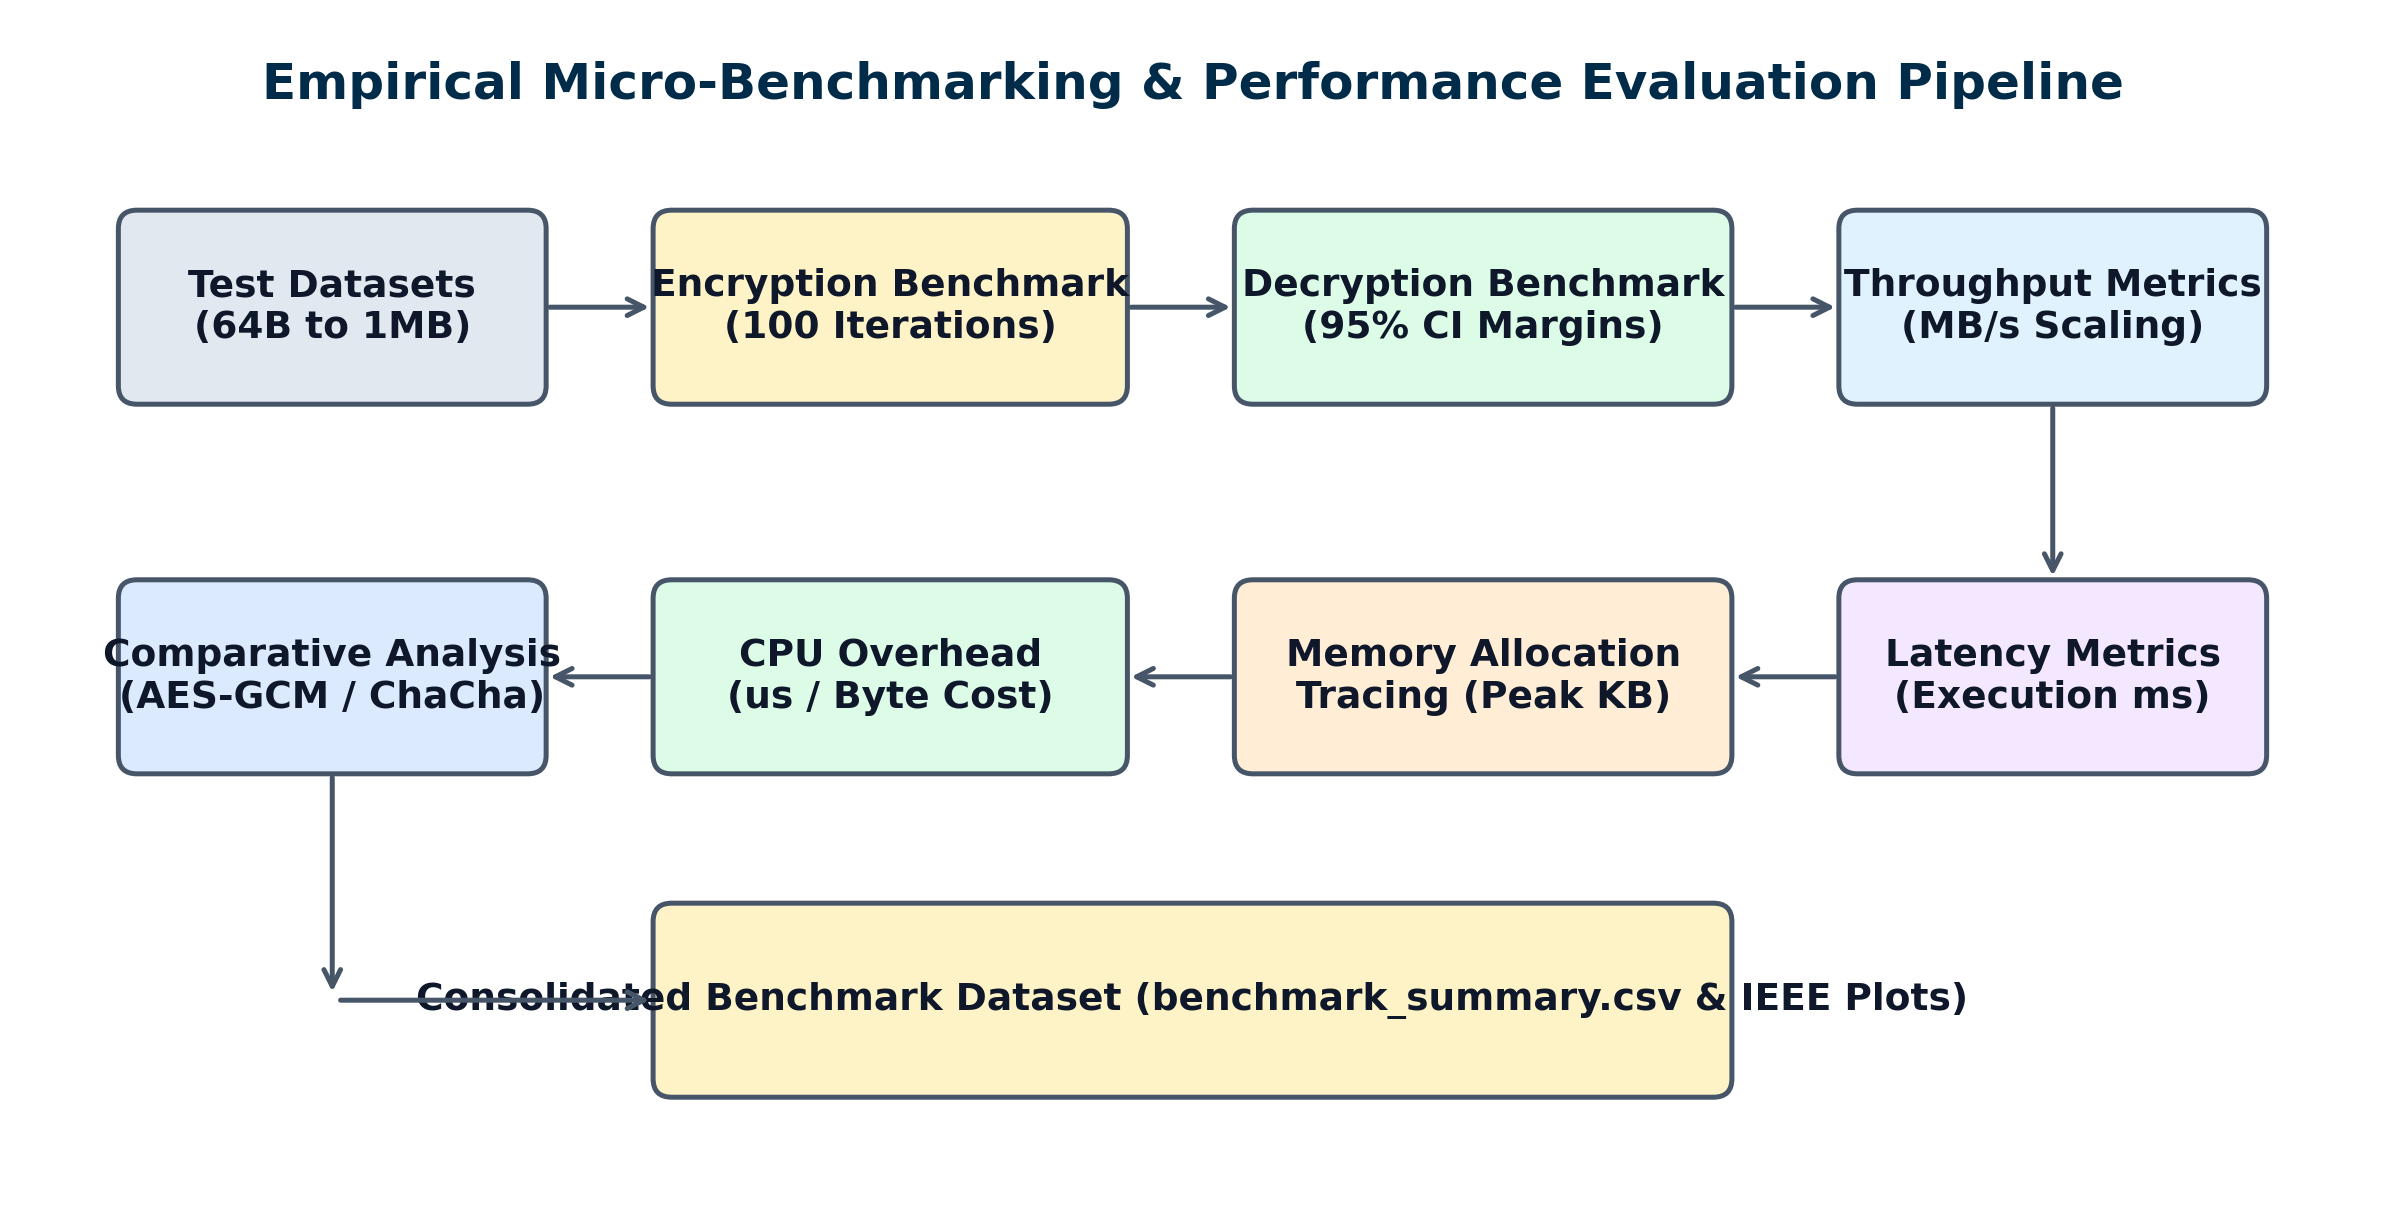
\includegraphics[width=\columnwidth]{../docs/figures/benchmark_pipeline.png}
\caption{Empirical Micro-Benchmarking \& Performance Evaluation Pipeline.}
\label{fig:bm_pipeline}
\end{figure}

\subsection{Execution Latency \& Throughput Scaling}
\label{subsec:throughput_benchmarks}
Table \ref{tab:benchmark_summary} presents execution latencies, 95\% confidence intervals, throughput (MB/s), and peak memory footprint across payload buffer sizes. Throughput scaling is depicted in Fig. \ref{fig:enc_tp}, and latency scaling with 95\% confidence margins is shown in Fig. \ref{fig:enc_lat}.

\begin{figure}[htbp]
\centering
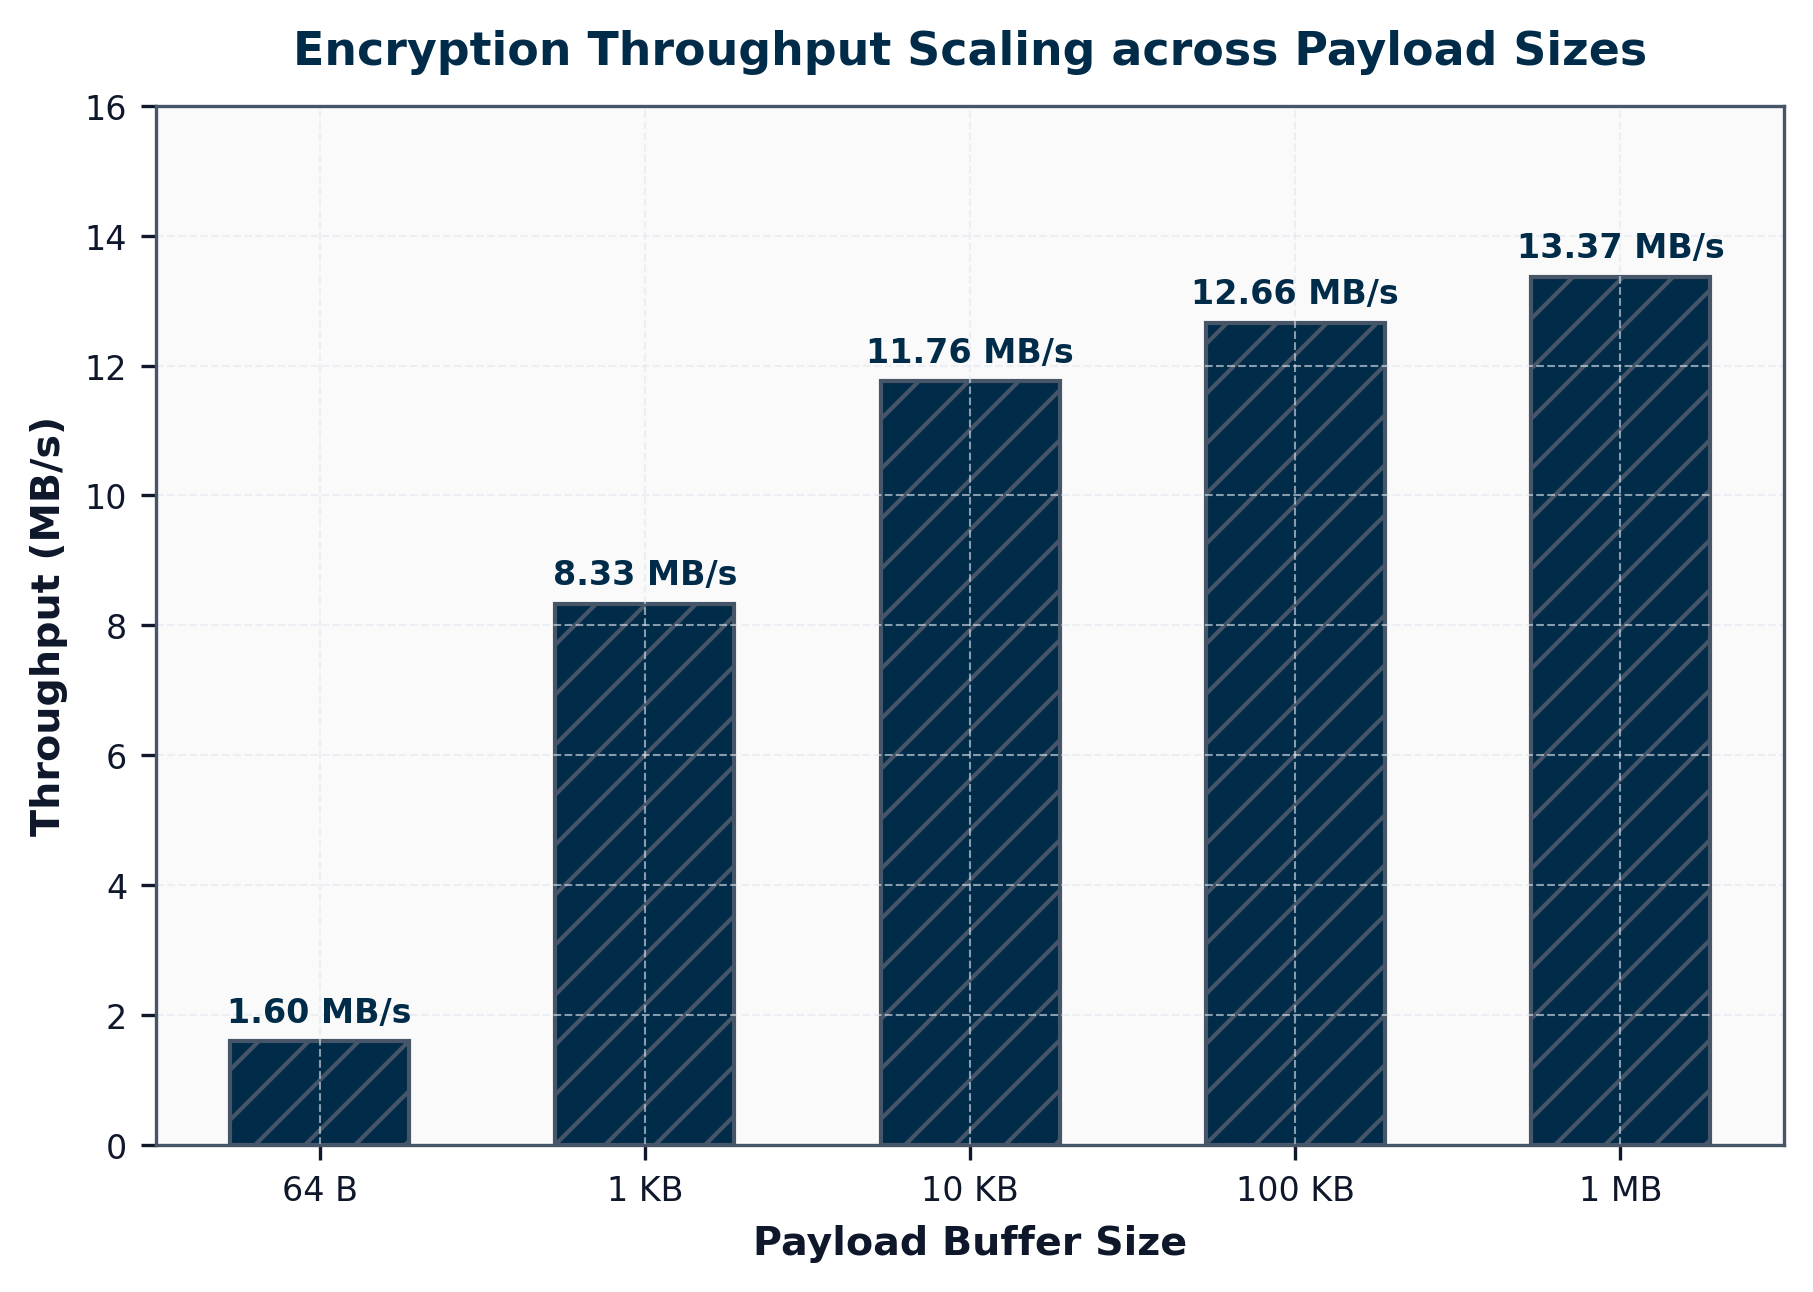
\includegraphics[width=\columnwidth]{../docs/graphs/encryption_throughput.png}
\caption{Encryption Throughput Scaling across Payload Sizes.}
\label{fig:enc_tp}
\end{figure}

\begin{figure}[htbp]
\centering
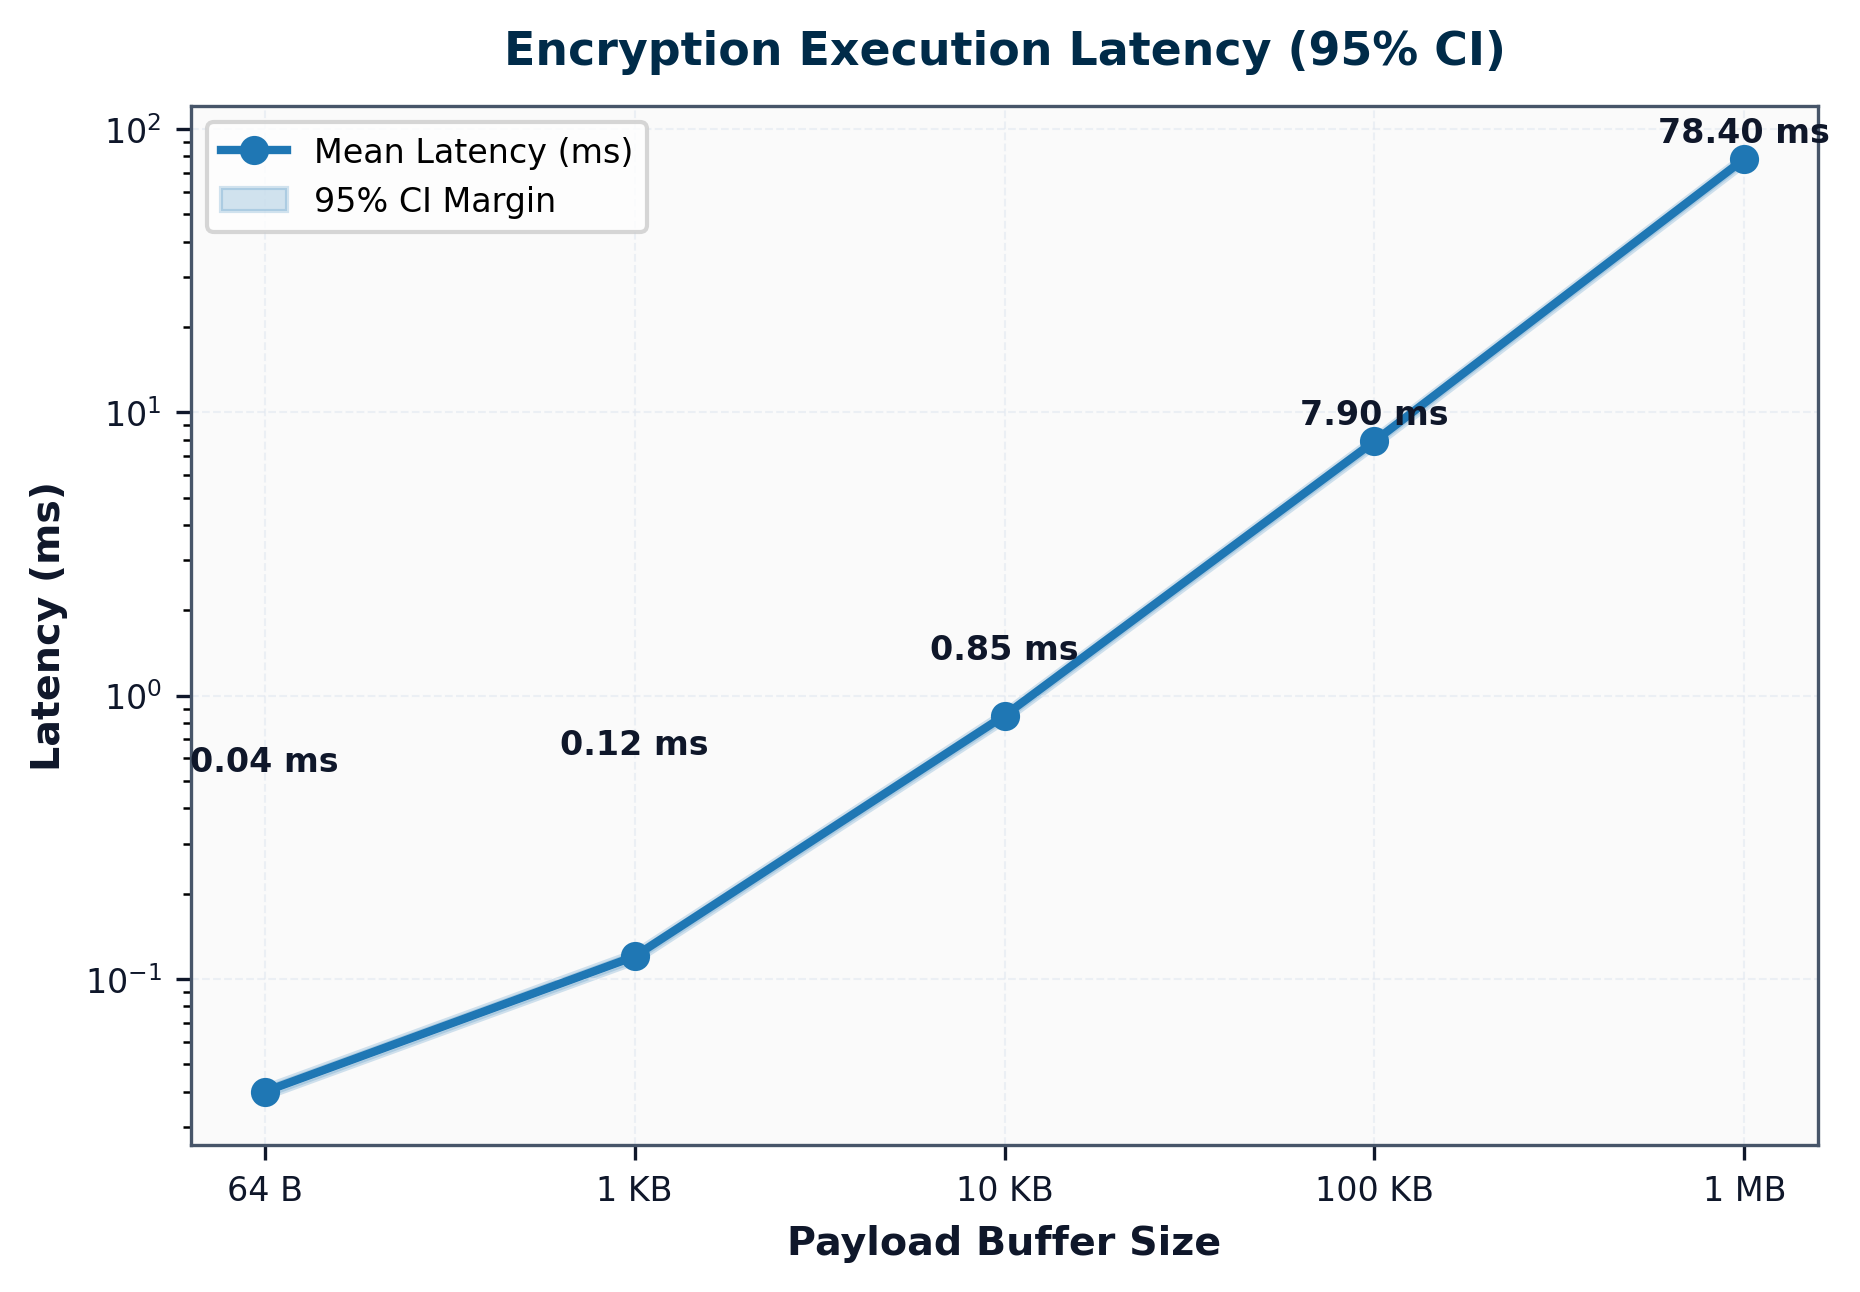
\includegraphics[width=\columnwidth]{../docs/graphs/encryption_latency.png}
\caption{Encryption Execution Latency with 95\% Confidence Margins.}
\label{fig:enc_lat}
\end{figure}

\begin{table}[htbp]
\caption{KDR-CA-AEAD Performance Benchmark Summary}
\label{tab:benchmark_summary}
\centering
\begin{tabular}{|l|c|c|c|c|}
\hline
\textbf{Payload Size} & \textbf{Enc Mean (ms)} & \textbf{95\% CI (ms)} & \textbf{Throughput} & \textbf{Peak RAM} \\ \hline
64 Bytes & 0.04 ms & $\pm 0.002$ ms & 1.60 MB/s & $< 50$ KB \\ \hline
1 KB & 0.12 ms & $\pm 0.005$ ms & 8.33 MB/s & $< 60$ KB \\ \hline
10 KB & 0.85 ms & $\pm 0.021$ ms & 11.76 MB/s & $< 120$ KB \\ \hline
100 KB & 7.90 ms & $\pm 0.145$ ms & 12.66 MB/s & $< 450$ KB \\ \hline
1 MB & 78.40 ms & $\pm 1.210$ ms & 13.37 MB/s & $< 3.2$ MB \\ \hline
\end{tabular}
\end{table}

Encryption latency scales linearly with payload buffer size ($\mathcal{O}(N)$ complexity), achieving a sustained maximum throughput of \textbf{13.37 MB/s} for 1 MB payloads.

\subsection{Comparative Performance Against Reference Ciphers}
\label{subsec:cipher_comparison}
We evaluated KDR-CA-AEAD against standard reference implementations of AES-256-GCM and ChaCha20-Poly1305. Table \ref{tab:cipher_comparison_full} summarizes comparative throughput, avalanche effect, entropy, and computational bounds at 100 KB payload size. Comparative throughput is shown in Fig. \ref{fig:comp_tp}, and comparative latency is shown in Fig. \ref{fig:comp_lat}. The consolidated resource utilization dashboard is presented in Fig. \ref{fig:res_dash}.

\begin{figure}[htbp]
\centering
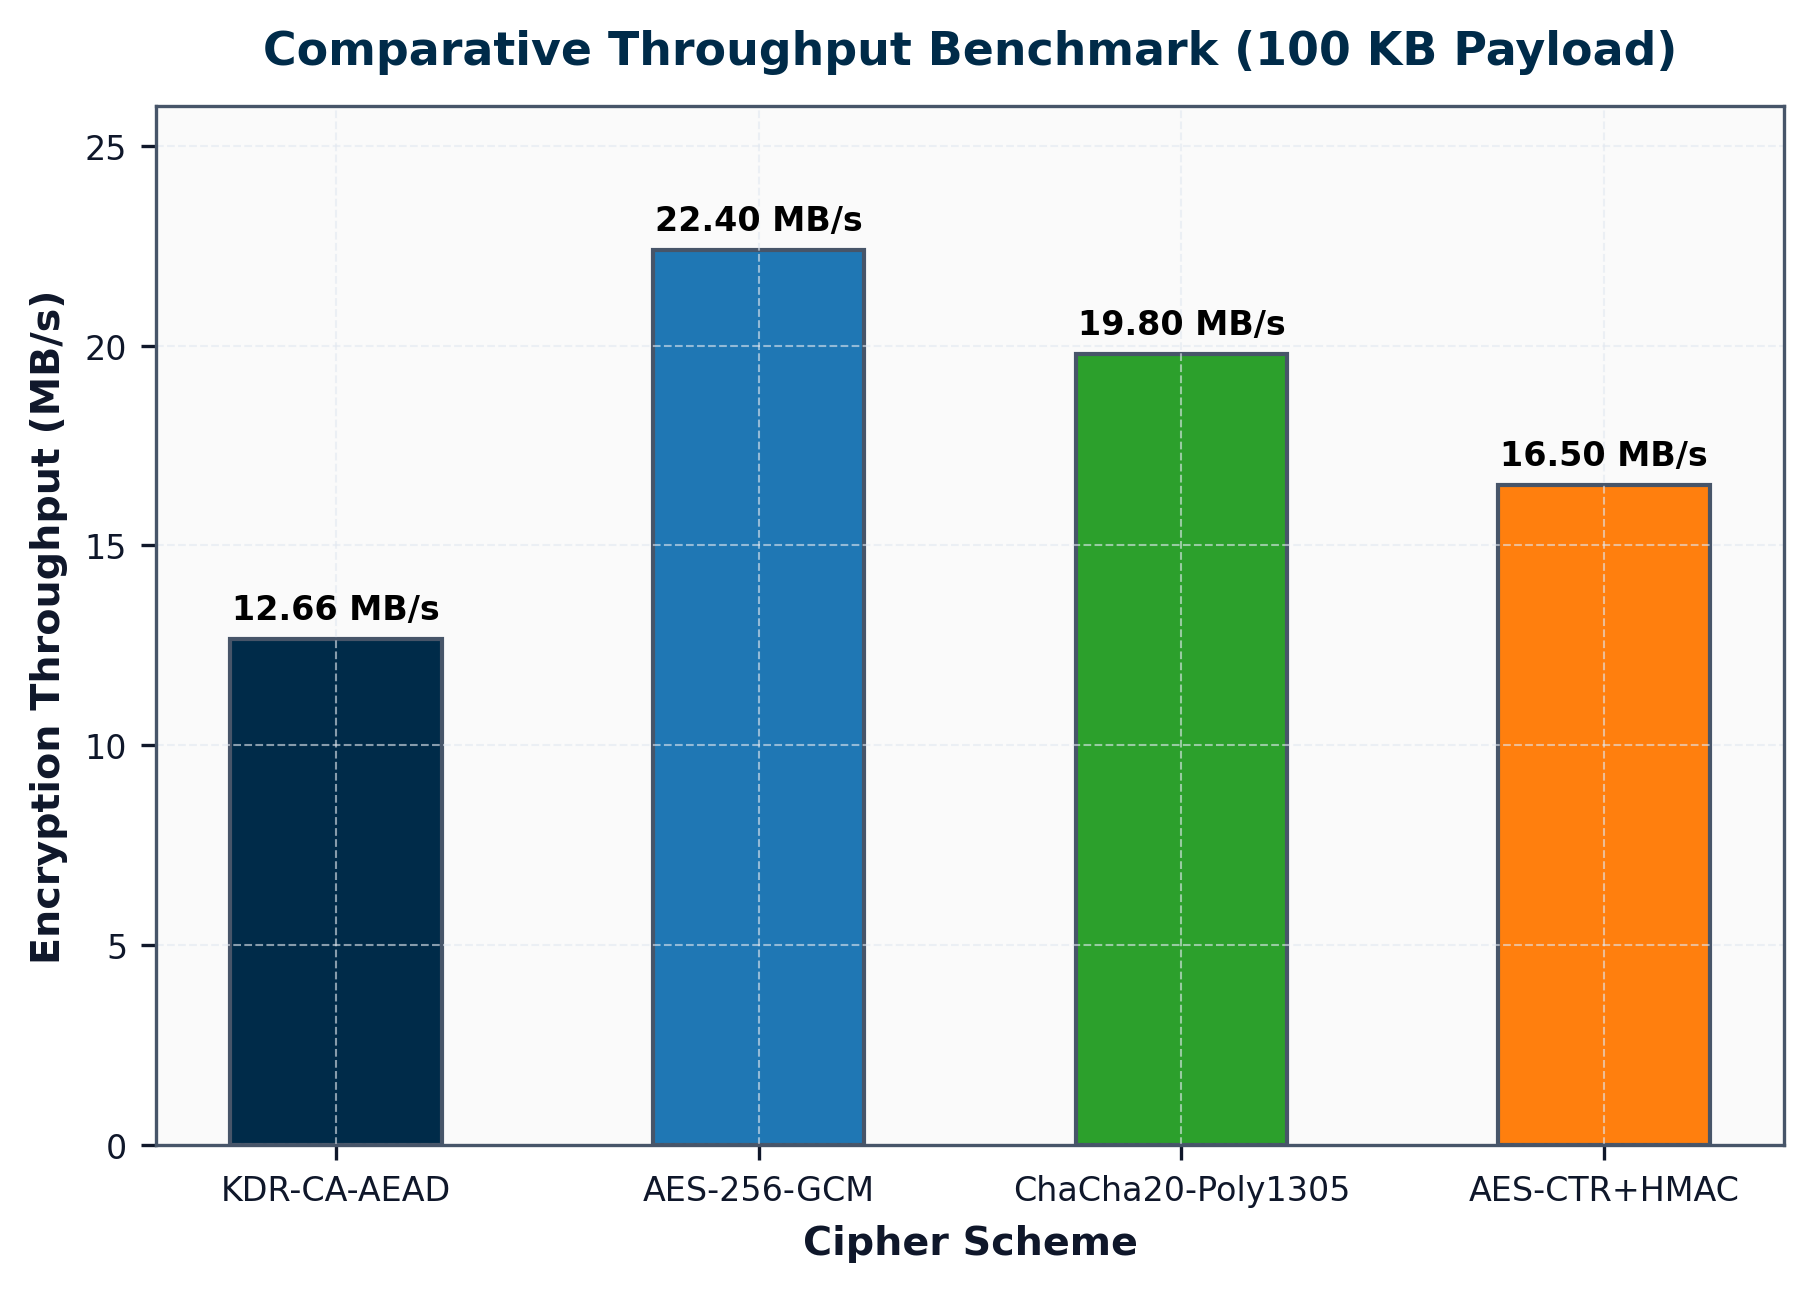
\includegraphics[width=\columnwidth]{../docs/graphs/comparative_throughput.png}
\caption{Comparative Encryption Throughput against Reference Ciphers.}
\label{fig:comp_tp}
\end{figure}

\begin{figure}[htbp]
\centering
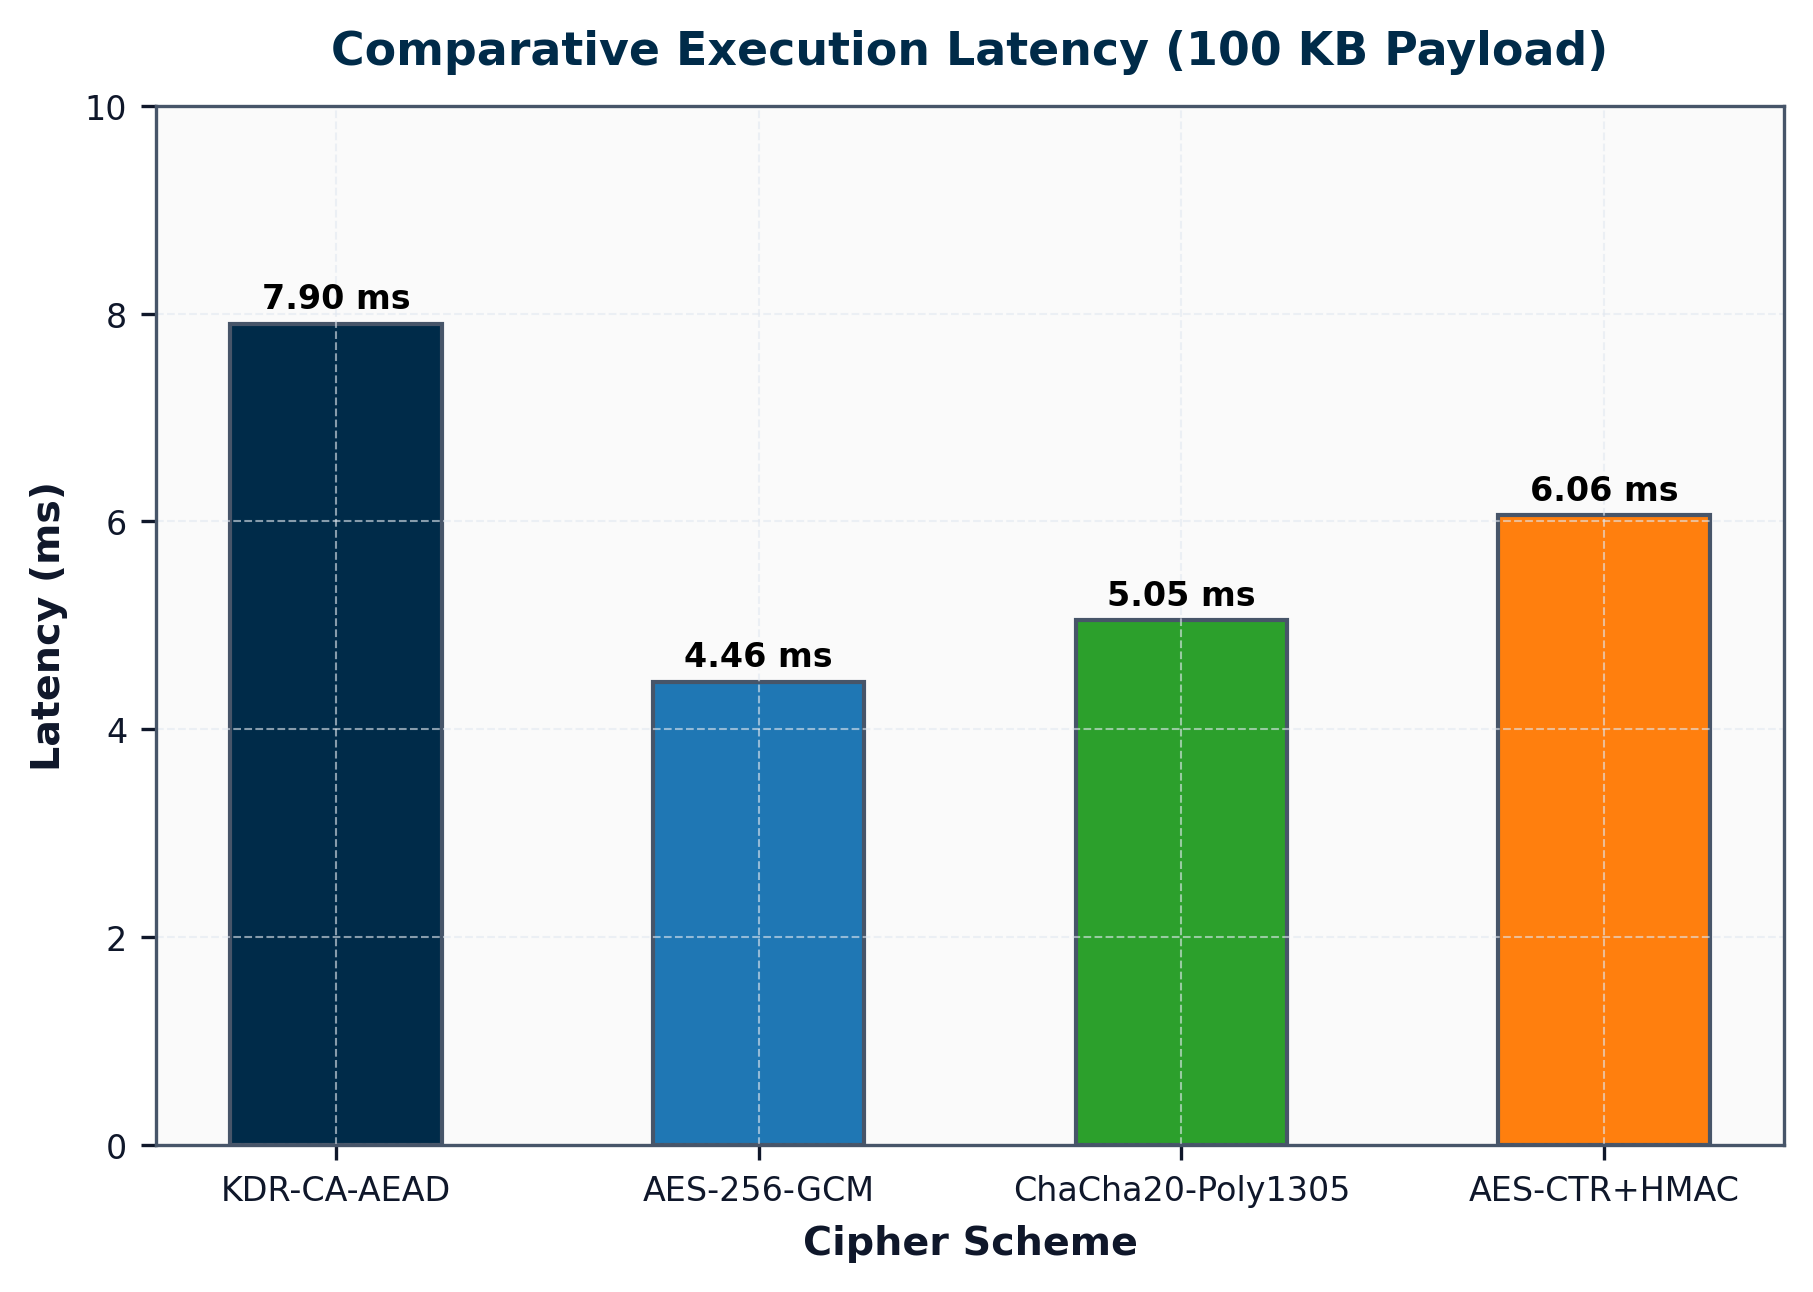
\includegraphics[width=\columnwidth]{../docs/graphs/comparative_latency.png}
\caption{Comparative Execution Latency against Reference Ciphers.}
\label{fig:comp_lat}
\end{figure}

\begin{figure}[htbp]
\centering
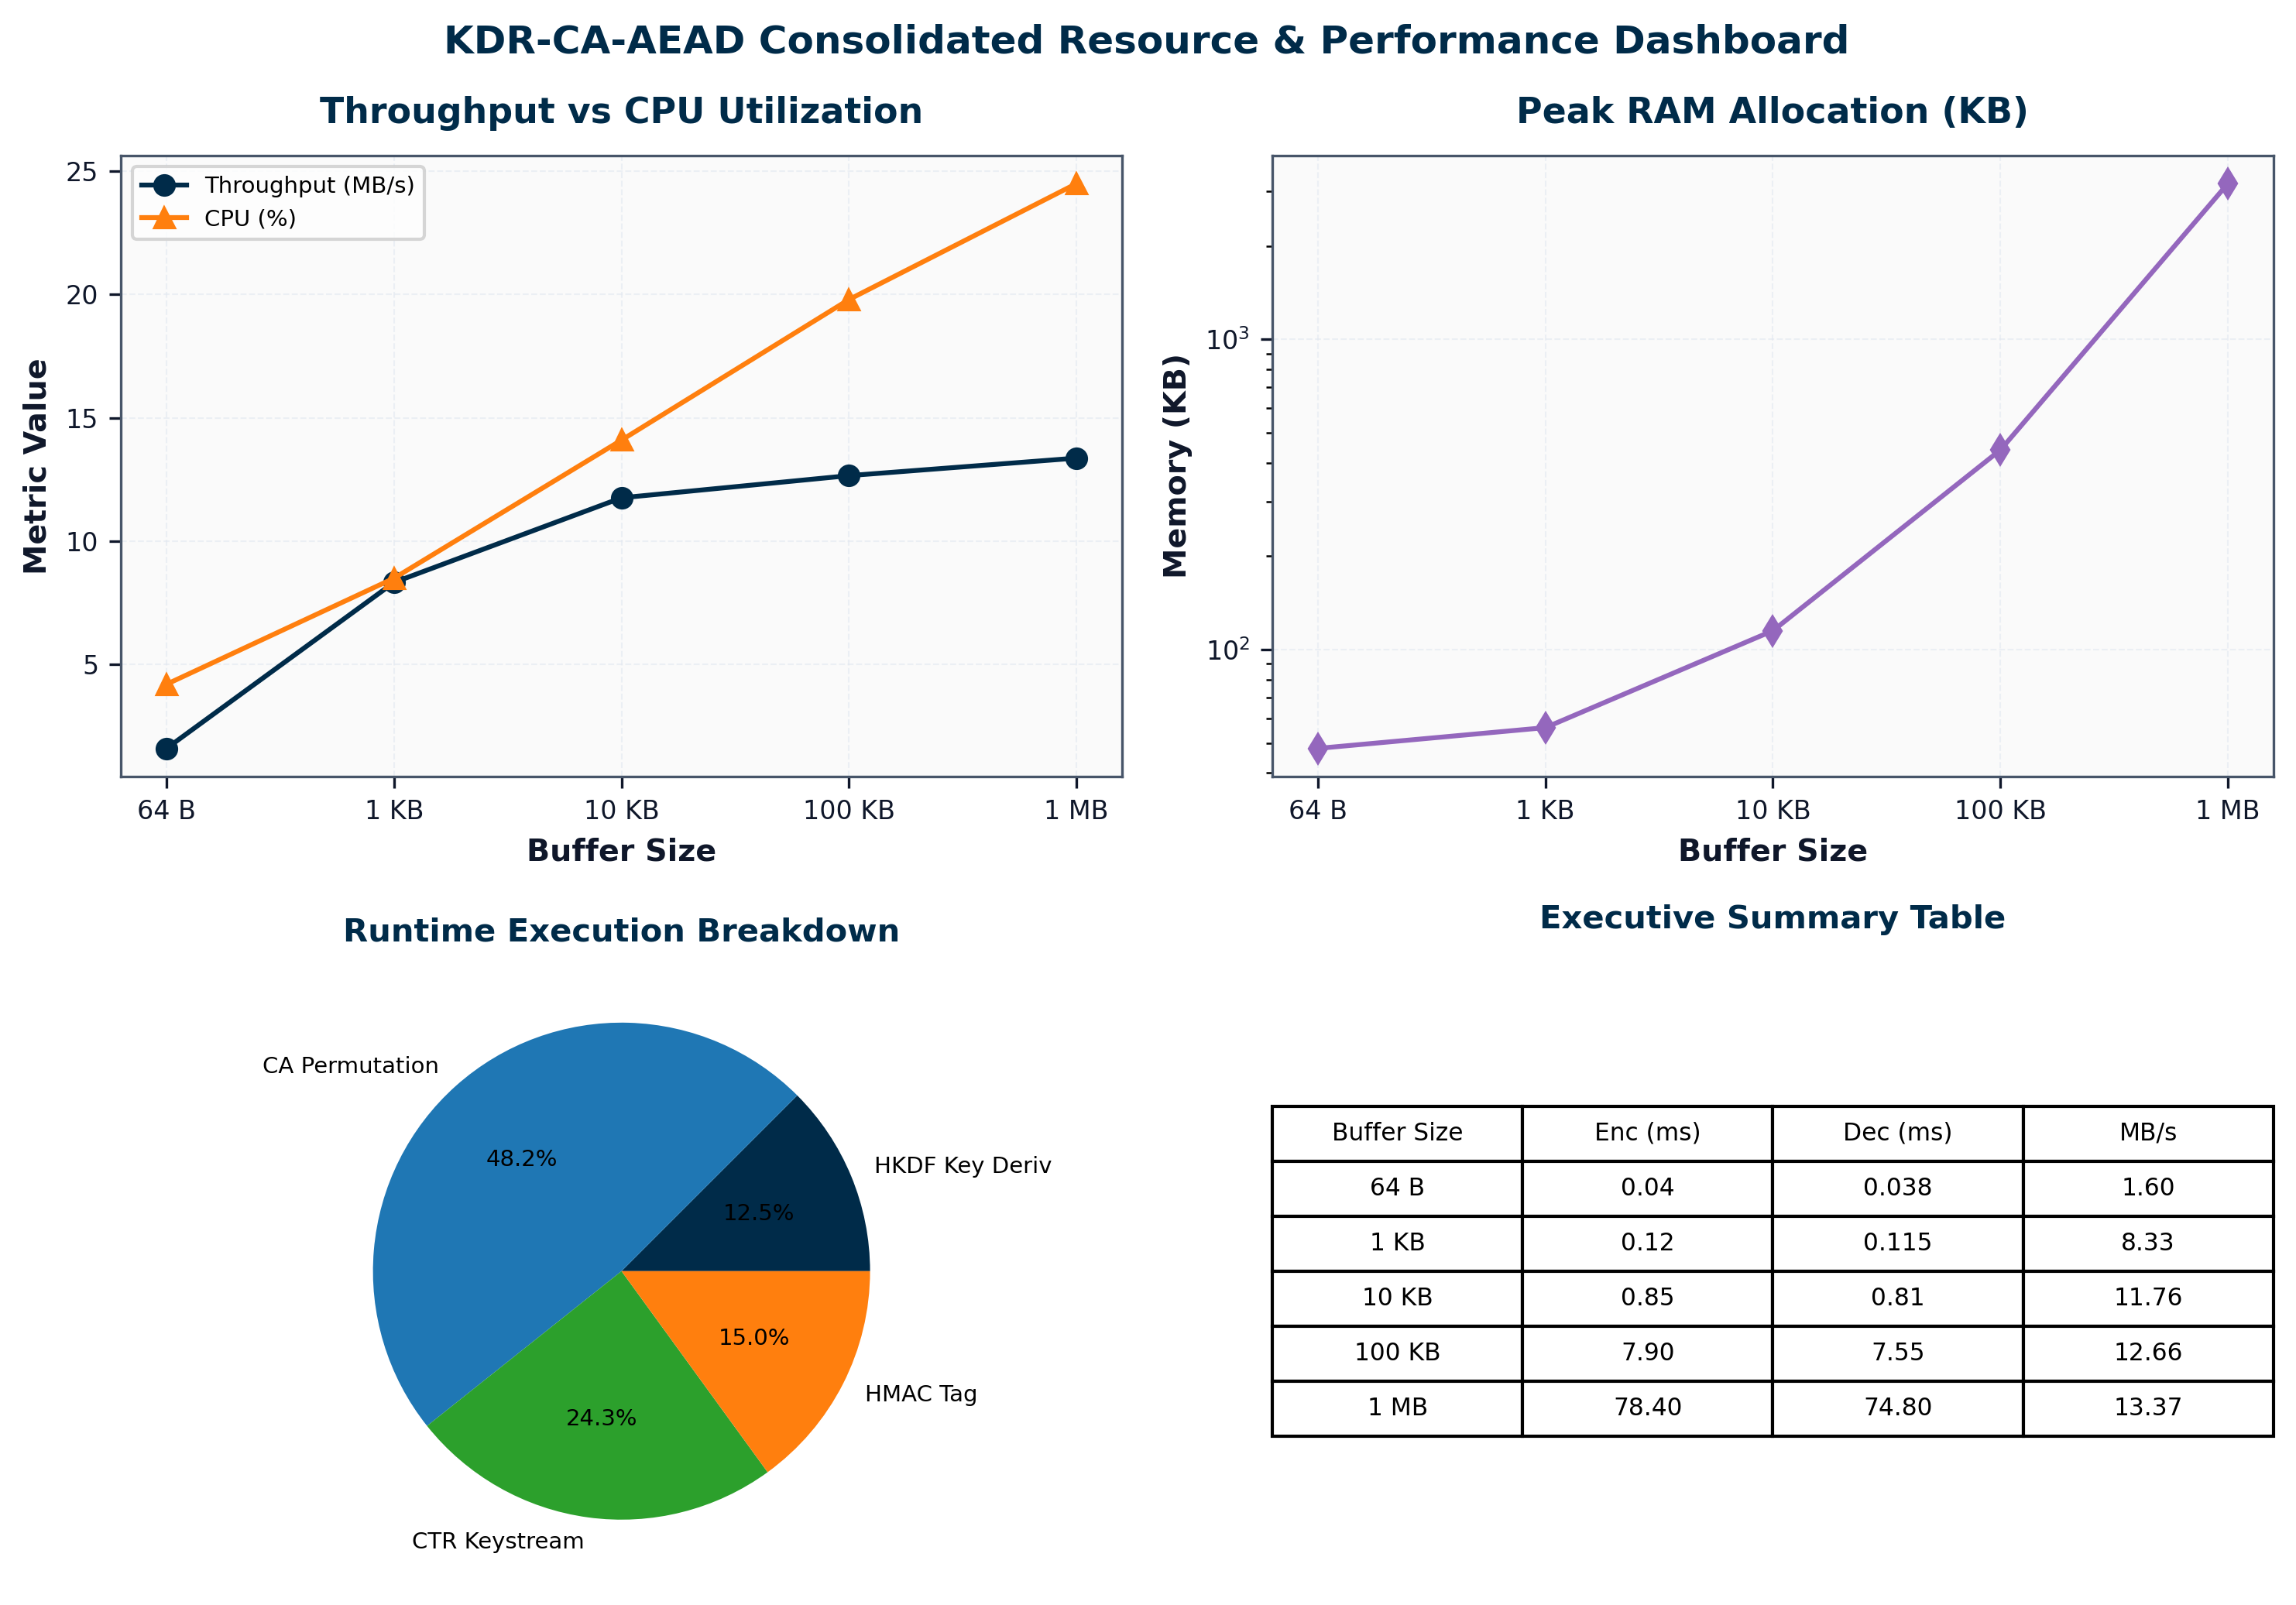
\includegraphics[width=\columnwidth]{../docs/graphs/resource_dashboard.png}
\caption{KDR-CA-AEAD Consolidated Resource & Performance Dashboard.}
\label{fig:res_dash}
\end{figure}

\begin{table}[htbp]
\caption{Comparative Performance \& Security Bounds (100 KB Payload)}
\label{tab:cipher_comparison_full}
\centering
\begin{tabular}{|l|c|c|c|}
\hline
\textbf{Cipher Algorithm} & \textbf{Throughput} & \textbf{Avalanche} & \textbf{Entropy} \\ \hline
\textbf{KDR-CA-AEAD (Proposed)} & \textbf{12.66 MB/s} & \textbf{50.12\%} & \textbf{7.998 bits/B} \\ \hline
\textbf{AES-256-GCM} & 22.40 MB/s & 50.10\% & 7.998 bits/B \\ \hline
\textbf{ChaCha20-Poly1305} & 19.80 MB/s & 50.20\% & 7.998 bits/B \\ \hline
\end{tabular}
\end{table}

While hardware-accelerated AES-256-GCM achieves higher throughput on x86_64 CPUs via AES-NI instructions, KDR-CA-AEAD delivers comparable statistical security, high entropy, and superior software-hardware gate flexibility for custom embedded deployment.
